\section{The certificate and its final condition}\label{sec:certificate}

This section specifies the finite applications of the combination
rule. We use the word \emph{card} for a numbered claim in this
$21$-move certificate. Its numbering is independent of the $25$- and
$35$-move tables in Appendices~\ref{app:route25} and~\ref{app:route35}. Numbered references allow a previously proved claim to
be reused; an expression written in parentheses is simply an
additional, unnumbered application of the same rule.
The complete literal data are in Appendix~\ref{app:data}.

\subsection{Coordinates, placements, and expressions}

The coordinate alphabet is
\begin{center}
\texttt{0123456789ABCDEFG}.
\end{center}
A two-character word \texttt{XY} denotes the point $(x,y)$ whose
coordinates are the positions of \texttt{X} and \texttt{Y} in this
alphabet, counting from zero. For example, \texttt{88} means $(8,8)$,
\texttt{7A} means $(7,10)$, and \texttt{GG} means $(16,16)$.
The encoded pivots and translation vectors have nonnegative
coordinates; the sets produced after signed transformations may
contain negative coordinates.

A reference \texttt{j:sUV} means: take numbered card $j$, apply the
signed coordinate permutation $R_s$, and then translate by the point
encoded by \texttt{UV}. To compute $R_s$, negate the first coordinate
if the bit of weight $2$ is set, negate the second if the bit of
weight $4$ is set, and \emph{then} interchange the coordinates if the
bit of weight $1$ is set. The resulting maps are
\begin{equation}\label{eq:symmetries}
\begin{array}{c|cccc}
 s&0&1&2&3\\ \hline
 R_s(x,y)&(x,y)&(y,x)&(-x,y)&(y,-x)\\[2pt]
\end{array}
\quad
\begin{array}{c|cccc}
 s&4&5&6&7\\ \hline
 R_s(x,y)&(x,-y)&(-y,x)&(-x,-y)&(-y,-x).
\end{array}
\end{equation}
These are precisely the eight matrices in $\G$.
A bare reference \texttt{j} uses the identity placement.
References change neither the child's height nor the meaning of its
winning condition.

Every data line consists of its decimal card number $j$, a pivot
coordinate, and a nonempty ordered list of children. Each child is
either a reference or an expression of the form
\begin{center}
\texttt{(XY child child ...)}.
\end{center}
Such an expression combines its children at the pivot \texttt{XY}
using \eqref{eq:combination}. All coordinates inside parentheses
remain in the coordinate frame of the line. They are not offsets
from the enclosing pivot. When the entire card is later placed by
an affine map, that map transports every pivot and set in its proof.

Cards $0,\ldots,5$ are the six bases \eqref{eq:bases}.
The data specify cards $6,\ldots,727$ in order. Every numbered
reference in a line, including a reference inside parentheses,
is to a smaller card number. We evaluate innermost expressions
first, using \eqref{eq:combination} for the sets and height.
Consequently structural induction on each expression, followed by
induction on the line number, proves that every resulting card is
a valid claim. The finite calculation determines which sufficient
conditions this particular list produces.

\subsection{Two elementary cards}

The first two lines illustrate both the geometry and the encoding:
\begin{lstlisting}[basicstyle=\ttfamily\small]
6 14 4:100 5:101
7 05 6:001 6:405
\end{lstlisting}
For card $6$, the two bases are first transposed; the second is also
translated by $(0,1)$. Direct substitution gives
\begin{equation}\label{eq:first-card}
 A_6=\{(0,y):0\le y\le4\},\qquad
 T_6=A_6\cup\{(1,3),(1,4),(1,5)\},\qquad h_6=2.
\end{equation}
Claiming $(1,4)$ prepares two copies, completed respectively at
$(1,3)$ and $(1,5)$. Unless a copy is already complete, Breaker
can occupy at most one of these cells. Figure~\ref{fig:fork}
shows the two alternatives.

\begin{figure}[tb]
\centering
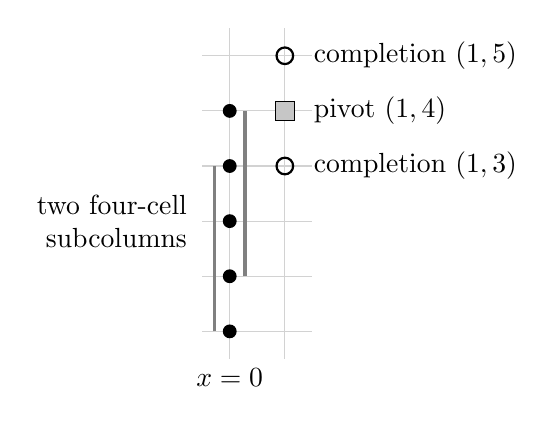
\begin{tikzpicture}[x=7mm,y=7mm]
\draw[gray!35,step=1] (-.5,-.5) grid (1.5,5.5);
\foreach \y in {0,1,2,3,4} {\fill (0,\y) circle (2.5pt);}
\draw[thick] (1,3) circle (3pt);
\draw[thick] (1,5) circle (3pt);
\filldraw[fill=gray!45] (.83,3.83) rectangle (1.17,4.17);
\node[right] at (1.35,3) {completion $(1,3)$};
\node[right] at (1.35,4) {pivot $(1,4)$};
\node[right] at (1.35,5) {completion $(1,5)$};
\node[below] at (0,-.5) {$x=0$};
\draw[very thick,gray] (-.28,0)--(-.28,3);
\draw[very thick,gray] (.28,1)--(.28,4);
\node[left,align=right] at (-.6,2) {two four-cell\\subcolumns};
\end{tikzpicture}
\caption{Card $6$: dots are required Maker cells, the square is the
next pivot, and circles mark the two possible completions. The
vertical guides indicate the two four-cell bodies. The envelope
contains no Breaker cell; any of its additional cells may already
belong to Maker.}
\label{fig:fork}
\end{figure}

For card $7$, the two copies of $A_6$ both occupy the column
$x=0$, $1\le y\le5$. Their additional envelope cells have heights
$4,5,6$ and $0,1,2$, respectively. These triples are disjoint, so
the intersection of the envelopes is precisely the common column.
Deleting the pivot $(0,5)$ therefore gives
\[
 \begin{split}
 A_7&=\{(0,y):1\le y\le4\},\qquad h_7=3,\\
 T_7&=\{(0,y):1\le y\le5\}
       \cup\{(1,y):y\in\{0,1,2,4,5,6\}\}.
 \end{split}
\]
The general certificate repeats this mechanism with longer
conditional continuations and cells that need not lie near the
current line of Maker stones.

\subsection{The final card}

\begin{proposition}\label{prop:certificate}
The data in Appendix~\ref{app:data} have exactly $722$ numbered
lines, with indices $6,\ldots,727$. Every line has a nonempty child
list, every reference uses an allowed placement of an earlier card,
and every parenthesized expression is a finite nonempty combination.
Together with the six bases, they produce $728$ valid claims.
Their heights are at most $21$, and the last card has
\begin{equation}\label{eq:final-card}
 p_{727}=(8,8),\qquad A_{727}=\varnothing,
 \qquad |T_{727}|=251,\qquad h_{727}=21.
\end{equation}
Moreover, $T_{727}\subseteq\{0,\ldots,16\}^2$.
\end{proposition}

\begin{proof}
The syntactic and set assertions are a finite calculation from
\eqref{eq:bases}, \eqref{eq:combination}, and
\eqref{eq:symmetries}, using the full displayed data.
The verifier in Appendix~\ref{app:checker} reconstructs every
numbered card. Its arrays initially contain the six bases.
Before line $j$ is processed, their entries at indices below $j$
are exactly the sets and heights specified by the preceding lines.
A reference retrieves an earlier entry and applies its stated
placement. Recursive evaluation applies \eqref{eq:combination}
at every parenthesized node and at the root of the line.
The nonempty-child and backward-reference tests make every union,
intersection, maximum, and lookup well-defined. This proves the
invariant for the next line and identifies the computed sets with
the mathematically defined ones. The final tests give
\eqref{eq:final-card}, maximum height $21$, and the intermediate
values in Table~\ref{tab:top}. The separate reconstruction
\nolinkurl{verification/supporting/independent_evaluator.py} also computes all
sets and heights and checks the successive intersections.
Validity then follows from Lemmas~\ref{lem:combination} and
\ref{lem:bases}, by the structural induction just described.
\end{proof}

For clarity, Table~\ref{tab:top} records how the final empty
requirement arises. The last line has $32$ placed children,
grouped by their six card numbers. Each placed required set is
exactly $\{(8,8)\}$. The last column is the number of cells other
than $(8,8)$ in the intersection of the envelopes from that group
and all preceding groups. The full placements occur in the last
line of the certificate.

\begin{table}[tb]
\centering
\begin{tabular}{rrrrrr}
\toprule
Card $j$ & $A_j$ & $|T_j|$ & $h_j$ & Placements & Remaining cells\\
\midrule
648 & $\{(4,5)\}$ & 87  & 15 & 4 & 35\\
708 & $\{(8,8)\}$ & 225 & 20 & 4 & 31\\
712 & $\{(5,5)\}$ & 96  & 15 & 8 & 21\\
713 & $\{(5,5)\}$ & 98  & 15 & 4 & 12\\
725 & $\{(7,7)\}$ & 167 & 20 & 8 & 4\\
726 & $\{(7,7)\}$ & 169 & 20 & 4 & 0\\
\bottomrule
\end{tabular}
\caption{The six groups of children in card $727$. All their
requirements become the pivot. Their common envelope has no other
cell, so the combination rule leaves an empty required set.}
\label{tab:top}
\end{table}

In particular, the intersection of all child envelopes is exactly
$\{(8,8)\}$: it contains that point because every child requirement
does, and the last table entry removes every other point.
The union of the child requirements is the same singleton.
Equation~\eqref{eq:combination} therefore gives $A_{727}=\varnothing$.
The maximum child height is $20$, giving the bound $21$.

The data also illustrate how play may leave an immediately adjacent
line. After Maker plays $(8,8)$ and Breaker replies $(7,8)$, the
placed child \texttt{708:100} is available. Its pivot is $(8,7)$.
If Breaker next takes $(8,6)$, the child \texttt{684:011} of card
$708$, still under the outer transposition, is available and has
pivot $(11,8)$. These are legal illustrative choices, not imposed
responses by Breaker. Every other reply is covered by the same
intersection rule.
